\documentclass[12pt,]{article}
\usepackage{lmodern}
\usepackage{amssymb,amsmath}
\usepackage{ifxetex,ifluatex}
\usepackage{fixltx2e} % provides \textsubscript
\ifnum 0\ifxetex 1\fi\ifluatex 1\fi=0 % if pdftex
  \usepackage[T1]{fontenc}
  \usepackage[utf8]{inputenc}
\else % if luatex or xelatex
  \ifxetex
    \usepackage{mathspec}
  \else
    \usepackage{fontspec}
  \fi
  \defaultfontfeatures{Ligatures=TeX,Scale=MatchLowercase}
\fi
% use upquote if available, for straight quotes in verbatim environments
\IfFileExists{upquote.sty}{\usepackage{upquote}}{}
% use microtype if available
\IfFileExists{microtype.sty}{%
\usepackage{microtype}
\UseMicrotypeSet[protrusion]{basicmath} % disable protrusion for tt fonts
}{}
\usepackage[margin=2.5cm]{geometry}
\usepackage{hyperref}
\hypersetup{unicode=true,
            pdftitle={Project 1: regression 1},
            pdfauthor={Urvan Christen, Amandine Goffeney, Joseph Vermeil, Lucile Vigué},
            pdfborder={0 0 0},
            breaklinks=true}
\urlstyle{same}  % don't use monospace font for urls
\usepackage{longtable,booktabs}
\usepackage{graphicx,grffile}
\makeatletter
\def\maxwidth{\ifdim\Gin@nat@width>\linewidth\linewidth\else\Gin@nat@width\fi}
\def\maxheight{\ifdim\Gin@nat@height>\textheight\textheight\else\Gin@nat@height\fi}
\makeatother
% Scale images if necessary, so that they will not overflow the page
% margins by default, and it is still possible to overwrite the defaults
% using explicit options in \includegraphics[width, height, ...]{}
\setkeys{Gin}{width=\maxwidth,height=\maxheight,keepaspectratio}
\IfFileExists{parskip.sty}{%
\usepackage{parskip}
}{% else
\setlength{\parindent}{0pt}
\setlength{\parskip}{6pt plus 2pt minus 1pt}
}
\setlength{\emergencystretch}{3em}  % prevent overfull lines
\providecommand{\tightlist}{%
  \setlength{\itemsep}{0pt}\setlength{\parskip}{0pt}}
\setcounter{secnumdepth}{0}
% Redefines (sub)paragraphs to behave more like sections
\ifx\paragraph\undefined\else
\let\oldparagraph\paragraph
\renewcommand{\paragraph}[1]{\oldparagraph{#1}\mbox{}}
\fi
\ifx\subparagraph\undefined\else
\let\oldsubparagraph\subparagraph
\renewcommand{\subparagraph}[1]{\oldsubparagraph{#1}\mbox{}}
\fi

%%% Use protect on footnotes to avoid problems with footnotes in titles
\let\rmarkdownfootnote\footnote%
\def\footnote{\protect\rmarkdownfootnote}

%%% Change title format to be more compact
\usepackage{titling}

% Create subtitle command for use in maketitle
\providecommand{\subtitle}[1]{
  \posttitle{
    \begin{center}\large#1\end{center}
    }
}

\setlength{\droptitle}{-2em}

  \title{Project 1: regression 1}
    \pretitle{\vspace{\droptitle}\centering\huge}
  \posttitle{\par}
    \author{Urvan Christen, Amandine Goffeney, Joseph Vermeil, Lucile Vigué}
    \preauthor{\centering\large\emph}
  \postauthor{\par}
      \predate{\centering\large\emph}
  \postdate{\par}
    \date{March 20, 2019}

\usepackage{fancyhdr}
\usepackage{wrapfig}
\pagestyle{fancy}
\fancyhead[LE,RO]{Christen, Goffeney, Vermeil, Vigu?f©}

\begin{document}
\maketitle

\subsection{Introduction}\label{introduction}

Mercury is a metal present in the environment whose harmful effects on
human health are well assessed (Park and Zheng 2012). In a study led in
2000 (Al-Majed and Preston 2000), scientists collected data on total
mercury and methyl mercury levels in the hair of 100 fishermen of
Kuwait, aged 16 to 58 years, comparing them to those of a control
population of 35 non-fishermen, aged 26 to 35 years. The aim of this
report is to analyse the factors influencing the levels of mercury in
both populations. For the sake of simplicity, we will only focus on
total Hg, leaving out methyl mercury, as both variables are strongly
correlated.

\begin{wrapfigure}{R}{0.35\textwidth}

\hfill{}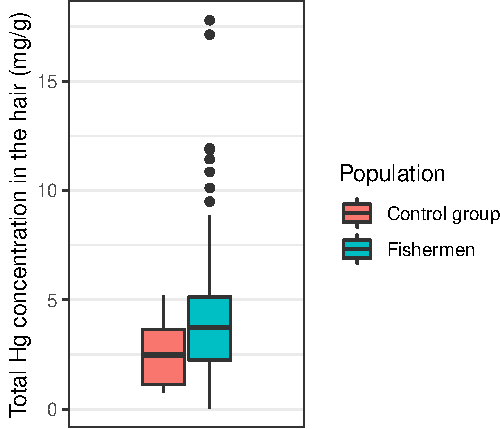
\includegraphics{Report_files/figure-latex/unnamed-chunk-4-1} 

\caption{Boxplots of Hg levels}\label{fig:unnamed-chunk-4}
\end{wrapfigure}

The dataset gathers information about six numerical variables (age,
height, weight, number of fish meals per week and residence time in
Kuwait) and two categorical ones (being a fisherman or not, fish
consumption habits). There is no additional information about gender as
all the participants in the study are males.

A first insight at the data shows that the fishermen population exhibits
higher levels of mercury in their hair. The significance of the
difference between the means of both distributions is assessed by a
\emph{Welch Two Sample t-test} with the alternative hypothesis that the
fishermen population has a average greater level of mercury than the
control population (\emph{p}-value = 7.473e-05).

\section{Exploratory analysis}\label{exploratory-analysis}

\subsubsection{Overview of the data}\label{overview-of-the-data}

Before fitting a model, let's have a look at the data. The following
table shows the 8 possible values of \emph{fishmlwk} according to the 2
possible values of \emph{fisherman}

\begin{longtable}[]{@{}lllllllll@{}}
\toprule
\textbf{Number of fish meal per week} & \textbf{0} & \textbf{1} &
\textbf{2} & \textbf{3} & \textbf{4} & \textbf{7} & \textbf{14} &
\textbf{21}\tabularnewline
\textbf{Fishermen} & 0 & 0 & 0 & 2 & 12 & 70 & 5 & 11\tabularnewline
\textbf{Non-fishermen} & 10 & 14 & 11 & 0 & 0 & 0 & 0 & 0\tabularnewline
\bottomrule
\end{longtable}

First, let's notice that for some values, we have a very few people, for
instance only 2 people eat fish 3 times a week. We see also that the
data is really unbalanced, because the \emph{fisherman} and the
\emph{fishmlwk} variable are very highly correlated: the non fishermen
don't eat fish more than 2 times a week, whereas the fishermen don't eat
fish less than 3 times a week. Besides, we face the same unbalanced
pattern for the variables \emph{age} and \emph{restime}.

\subsubsection{Multicolinearity}\label{multicolinearity}

To check whether we have multicolinear variables, we use the variance
inflation factor (VIF). We set the following criteria: we keep only the
variables that have a result below 5. We observe that all the variables
have a variance inflation factor below 2, so we don't eliminate any
variable, yet.

\subsection{Model selection}\label{model-selection}

Now we are going to use and compare the different methods of model
selection to select the more relevant parameters to explain the TotHg
variations within the population.

\subsubsection{Stepwise selection}\label{stepwise-selection}

The first attempt is a stepwise selection based on a formula with all
the parameters except for \emph{fisherman}. Indeed, the preliminary
exploration has shown that the \emph{fisherman} variable have
considerable impact on many of the other variables. Therefore to
understand what is the reason behind the TotHg difference between the 2
groups, it seems natural to start with a model without the
\emph{fisherman} variable.

\begin{verbatim}
##                Estimate Std. Error   t value     Pr(>|t|)
## (Intercept) -10.0768196 2.44480942 -4.121720 6.603741e-05
## weight        0.1751823 0.03322237  5.273023 5.336914e-07
## fishmlwk      0.1588378 0.04174543  3.804915 2.161017e-04
\end{verbatim}

With stepwise selection, the selected model is : TotHg \textasciitilde{}
weight + fishmlwk. The intercept and the two coefficients are very
significant. Moreover the signs of the coefficients are not absurd:
while it is not really intuitive that the weight coefficient should be
positive or negative, the coefficient of \emph{fishmlwk} had to be
positive, and it's the case here.

Now to determine possible differences between the fishermen and
non-fishermen, a model based on the interactions between the
\emph{fisherman} variable and all the others is proposed. This could
show if a certain variable is very relevant concerning fishermen but
less when it comes to non-fishermen, for instance. We also include the
\emph{fisherman} variable itself, that will allow to include an
adjustment term between the values of the intercepts of the two groups
if it is relevant.

\begin{verbatim}
##                        Estimate Std. Error    t value     Pr(>|t|)
## (Intercept)         -1.41565206 6.93853651 -0.2040275 8.386536e-01
## fisherman1          -8.99967794 7.42906339 -1.2114149 2.279509e-01
## fisherman0:weight    0.03313256 0.09907139  0.3344312 7.385973e-01
## fisherman1:weight    0.18908832 0.03644361  5.1885177 8.003708e-07
## fisherman0:fishmlwk  1.53107486 0.70200877  2.1809911 3.099742e-02
## fisherman1:fishmlwk  0.09828757 0.05265742  1.8665473 6.423521e-02
\end{verbatim}

The best model is now : TotHg \textasciitilde{} fisherman +
fisherman:weight + fisherman:fishmlwk. While the coefficients for
fisherman1:weight and fisherman0:fishmlwk stays very significant,
fisherman1:fishmlwk is barely significant and fisherman0:weight,
fisherman1 and the intercept are far from being significant. Moreover,
when looking at the values of the coefficients, it appears that for the
non-fishermen, the number of fish meal per week has a very preponderant
(and reliable) effect compared to the weight influence, while among
fishermen, the contribution of weight is twice the one of fish meal per
week. Eventually the value of the fisherman1 parameter is surprising: it
implies that the fact of being a fisherman gives you -8.99 mg/g Hg. Yet
this comes from the increased value of fisherman1:weight, which will
make the overall Hg concentration more important among fishermen, as
expected.

In order to check the dependency of the selected model to the selection
technique, we have tried backward and forward selection and obtained
similar models.

\subsection{Results and discussion}\label{results-and-discussion}

Fit model (* fishermen) (I picked the model given by stepwise selection)

\begin{verbatim}
##                         Estimate Std. Error    t value     Pr(>|t|)
## fisherman0           -1.41565206 6.93853651 -0.2040275 8.386536e-01
## fisherman1          -10.41533001 2.65474931 -3.9232819 1.412643e-04
## fisherman0:weight     0.03313256 0.09907139  0.3344312 7.385973e-01
## fisherman1:weight     0.18908832 0.03644361  5.1885177 8.003708e-07
## fisherman0:fishmlwk   1.53107486 0.70200877  2.1809911 3.099742e-02
## fisherman1:fishmlwk   0.09828757 0.05265742  1.8665473 6.423521e-02
\end{verbatim}

This regression shows several interesting results:

\subsubsection{Difference between fisherman and control
populations}\label{difference-between-fisherman-and-control-populations}

First, we get two coefficients very significantly different from 0
(\emph{p} \textless{} 0.001), both concerning fisherman population. The
fact that there are less significant coefficients for non-fisherman
population could be explained by several causes:

\begin{itemize}
\tightlist
\item
  The non-fisherman population could be too small to properly show the
  size effect of those observables.
\item
  The non-fisherman population may not have settled long enough in the
  place to have repercussion on the mercury levels.
\end{itemize}

However, those are only suppositions in order to explain the
distribution of the \emph{p}-values, but none of them have been proven.
Further experiments are needed in order to show whether or not those
observables have a really different effect on both populations.

\subsubsection{Number of fish meals per
week}\label{number-of-fish-meals-per-week}

On the other side, the number of meal composed of fish (\emph{fishmlwk})
seems to be contributing to the mercury levels of both populations
(\emph{p}-values of 0.03 for non-fisherman and 0.06 for fisherman).
However, we can see that there is a huge difference between the two
contributions of a factor 16.

Here again, we can come up with some possible explanations, needing
further inquiries:

\begin{itemize}
\item
  The distribution of \emph{fishmlwk} is very different between both
  populations and thus may lead to different coefficients if the effect
  of this observables is not truly linear (\emph{e.g.} a logarithmic
  effect that could take some ceiling effects into account, \emph{i.e.}
  the fact that past a certain dose, the hair cannot absorb more
  mercury).
\item
  The observables does not reflect entirely the quantity of fish eaten,
  since one can eat more or less fish per meal. The weight of fish eaten
  per week, might be a more accurate observable to study.
\end{itemize}

Here again, more expriements are required to confirm or reject those
hypotheses.

\subsubsection{Weight}\label{weight}

However, the most significant coefficient is for \emph{weight} for
fisherman population, with a \emph{p}-value of 8e-07. This coefficient
suggest a high positive correlation between the weight of the fisherman
and the concentration of mercury in its hair.

The fact that the weight has a positive influence on this concentration
was unexpected, since a concentration and not an absolute quantity was
measured.

However, even though it was unexpected it has many possible explanations
such as the fact that weight is much likely correlated with adiposity
more susceptible to catch toxins than other tissues. Another explanation
could be that the fatter, the more one eats and possibly ingests mercury
that could fix in the hair; since hair weight isn't likely to be
correlated with body weight, it could explain the high mercury
concentration in hair.

Here again, further experiments are needed in order to support or reject
those hypotheses.

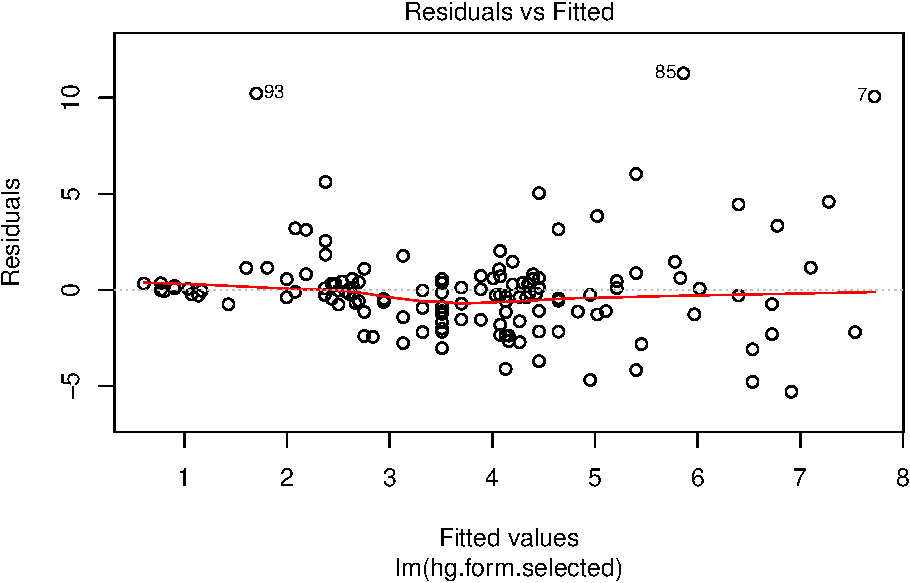
\includegraphics{Report_files/figure-latex/unnamed-chunk-16-1.pdf} The
model does not seem to be really homoscedastic. Variance is much higher
for fishermen than for non-fishermen. However, within each class, the
variance is overall well distributed, even if it tends to be a little
more spread for high fitted values. But, since our model is split into
two submodels corresponding to fisherman population and non-fisherman
population, the difference of variances between both classes doesn't
matter.

\includegraphics{Report_files/figure-latex/unnamed-chunk-17-1.pdf}

We have a heavy tails distribution of residuals, with a very heavy right
tail. The fact that we have two submodels merged in one might explain
the heavy tails. However it cannot explain the difference between right
and left tails. This could be caused by an insufficient sample size. Or
it could be explained by a non-linear relation between the observables
and the concentration of mercury, thus possibly unbalancing the
residuals distribution.

\subsection{Conclusion}\label{conclusion}

We have achieved to build a simple model that can help explaining the
levels of mercury observed in a fishermen population compared to a
control group. It appears that the variables that have the most
significant influence over the measured levels of mercury are the weight
of the individual and the frequency at which they eat fish. The former
can seem surprising even if some hypotheses can be formed to account for
the influence of weight on mercury levels. The latter may be the main
explanation for the differences observed between our two groups:
fishermen use to eat fish much more often than non-fishermen, as fish is
a well-known source of mercury it seems logical to see a positive
correlation between fish meal frequency and mercury levels and thus to
observe higher mercury levels in fishermen populations compared to
non-fishermen.

\subsection*{References}\label{references}
\addcontentsline{toc}{subsection}{References}

\hypertarget{refs}{}
\hypertarget{ref-al2000factors}{}
Al-Majed, NB, and MR Preston. 2000. ``Factors Influencing the Total
Mercury and Methyl Mercury in the Hair of the Fishermen of Kuwait.''
\emph{Environmental Pollution} 109 (2). Elsevier: 239--50.

\hypertarget{ref-park2012human}{}
Park, Jung-Duck, and Wei Zheng. 2012. ``Human Exposure and Health
Effects of Inorganic and Elemental Mercury.'' \emph{Journal of
Preventive Medicine and Public Health} 45 (6). Korean Society for
Preventive Medicine: 344.


\end{document}
